\setcounter{chapter}{0}
\chapter{INTRODUCTION}
Example of \textbf{Acronym[\acs{A}]}. 

\section{Example of section} 
In this section is presented a example of citations \cite{article}.

Example of Figure \ref{fig:figure1}. 
\begin{figure}[H]
	\centering
	{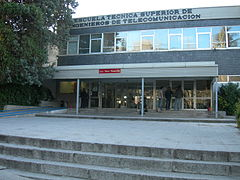
\includegraphics[width=.55\textwidth]{UPM-ETSIT--Sanz_Mancebo} }
	\caption{Figure 1}%
	\label{fig:figure1}
\end{figure}
Example of two figures:
\begin{figure}[h!]
	\centering
	\subfloat[Subtitle 1]{{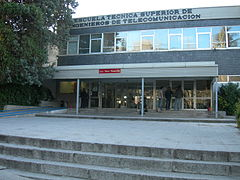
\includegraphics[width=.45\textwidth]{UPM-ETSIT--Sanz_Mancebo} }} \label{fig:subfigure1}
	\qquad
	\subfloat[Subtitle 2]{{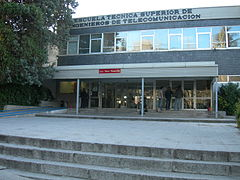
\includegraphics[width=.45\textwidth]{UPM-ETSIT--Sanz_Mancebo} }} \label{fig:subfigure2}
	\caption{Figure 2}%
	\label{fig:figure2}
\end{figure}

Example of table:
\begin{table}[H]
	\begin{center} {\footnotesize
			\begin{tabularx}{\textwidth}{@{} lXlX @{} }
				\multicolumn{2}{c}{} \\ 
				\hline
				
				\normalsize \textbf{Label} & \normalsize \textbf{values} \\

				\hline
				& \\
				label  & Description\\
				& \\
				label  & Description\\
				\hline
		\end{tabularx}}
	\end{center}
	\caption{\footnotesize Table 1}
	\label{table1}
\end{table}

\section{Example of section}
Example of list:
\renewcommand\labelitemi{\ding{117}}
\begin{itemize}
	\item First.
	\item Secondly.
	\item In the third place.
	\item Chapter 4.
	\item Last but not least.

\end{itemize}